\documentclass[handout]{mcs}

\begin{document}

\inclassproblems{2, Mon.}

%%%%%%%%%%%%%%%%%%%%%%%%%%%%%%%%%%%%%%%%%%%%%%%%%%%%%%%%%%%%%%%%%%%%%
% Problems start here
%%%%%%%%%%%%%%%%%%%%%%%%%%%%%%%%%%%%%%%%%%%%%%%%%%%%%%%%%%%%%%%%%%%%%

\begin{problem}
Prove by truth table that $\QOR$ distributes over $\QAND$:
\begin{equation}\label{dist}
\brac{A \; \QOR\ (B\ \QAND\ C)} \quad\text{is equivalent to}\quad
\brac{(A\ \QOR\ B)\ \QAND\ (A\ \QOR\ C)}
\end{equation}

\begin{solution}

\[
\begin{array}{|c|c|ccc|}
\hline
\text{[}A      & \QOR  & \text{(}B    & \QAND & C\text{)]}   \\ \hline
\true  &\true       & \true  & \true      & \true \\ \hline
\true  &\true       & \true  & \false     & \false\\ \hline
\true  &\true       & \false & \false     & \true \\ \hline
\true  &\true       & \false & \false     & \false\\ \hline
\false &\true       & \true  & \true      & \true \\ \hline
\false &\false      & \true  & \false     & \false\\ \hline
\false &\false      & \false & \false     & \true \\ \hline
\false &\false      & \false & \false     & \false\\ \hline
\end{array}
\]

\[
\begin{array}{|ccc|c|ccc|}
\hline
\text{[(}A  & \QOR      & B\text{)} & \QAND       & \text{(}A & \QOR      & C\text{)]} \\  \hline
     \true  & \true     & \true     & \true      &   \true   & \true     & \true \\  \hline
     \true  & \true     & \true     & \true      &   \true   & \true     & \false\\  \hline
     \true  & \true     & \false    & \true      &   \true   & \true     & \true \\  \hline
     \true  & \true     & \false    & \true      &   \true   & \true     & \false\\  \hline
     \false & \true     & \true     & \true      &   \false  & \true     & \true \\  \hline
     \false & \true     & \true     & \false     &   \false  & \false    & \false\\  \hline
     \false & \false    & \false    & \false     &   \false  & \true     & \true \\  \hline
     \false & \false    & \false    & \false     &   \false  & \false    & \false\\  \hline
\end{array}
\]

\end{solution}


\end{problem}

\insolutions{\newpage}
\begin{problem} 
\label{sys}
This problem\footnote{From Rosen, 5th edition, Exercise 1.1.36} examines
whether the following specifications are satisfiable:

\begin{enumerate}

\item If the file system is not locked, then

   \begin{enumerate}

   \item new messages will be queued.

   \item new messages will be sent to the messages buffer.

   \item the system is functioning normally, and conversely, if the system
         is functioning normally, then the file system is not locked.

   \end{enumerate}

\item  If new messages are not queued, then they will be sent to
the messages buffer.

\item  New messages will not be sent to the message buffer.

\end{enumerate}

\bparts

\ppart Begin by translating the five specifications into
propositional formulas using four propositional variables:
\begin{eqnarray*}
L   & \eqdef &   \text{file system locked}, \\
Q   & \eqdef &   \text{new messages are queued}, \\
B   & \eqdef &   \text{new messages are sent to the message buffer}, \\
N   & \eqdef &   \text{system functioning normally}.
\end{eqnarray*}

\begin{solution}

The translations of the specifications are:
\begin{align}
\QNOT L  \QIMPLIES & Q & \tag{Spec.\ 1.(a)}\\
\QNOT L  \QIMPLIES & B & \tag{Spec.\ 1.(b)}\\
\QNOT L  \QIFF  & N & \tag{Spec.\ 1.(c)}\\
\QNOT Q  \QIMPLIES & B & \tag{Spec.\ 2.}\\
\QNOT B           &   & \tag{Spec.\ 3.}
\end{align}
\end{solution}

\ppart\label{assign} Demonstrate that this set of specifications is
satisfiable by describing a single truth assignment for the variables
$L,Q,B,N$ and verifying that under this assignment, all the specifications
are true.

\begin{solution}
An assignment that works is
\begin{eqnarray*}
L       & = &   \true \\
N       & = &   \false \\
Q       & = &   \true \\
B       & = &   \false.
\end{eqnarray*}

To find this assignment, we could have started constructing the sixteen
line truth table ---one line for each way of assigning truth values to the
four variables $L$, $N$, $Q$, and $B$ ---and calculated the truth value of
the AND of all the five specifications under that assignment, continuing
until we got one that made the $\QAND$-formula true.

If for every one of the sixteen possible truth assignments, the
$\QAND$-formula was false, then the system is not satisfiable.
\end{solution}

\ppart Argue that the assignment determined in
part~\eqref{assign} is the only one that does the job.

\begin{solution}
We can avoid calculating all 16 rows of the full truthtable
  calculation suggested in the previous solution to part~\eqref{assign} by
  reasoning as follows.  In any truth assignment that makes all five
  specifications true,
\begin{itemize}

\item $B$ must be false, or the last specification, (Spec.\ 3.), would be
false.

\item Given that $B$ is false, (Spec.\ 2.) and (Spec.\ 1.(b)) can be
true only if $Q$ and $L$ are true.

\item Given that $L$ is true, (Spec.\ 1.(c)) can
be true only if $N$ is false.

\end{itemize}
Thus, in order for all five specifications to be true, the assignment must be:
\begin{eqnarray*}
L       & = &   \true \\
N       & = &   \false \\
Q       & = &   \true \\
B       & = &   \false.
\end{eqnarray*}

\end{solution}

\eparts
\end{problem}

\iffalse

\begin{problem}
\bparts

\ppart A propositional formula is \term{valid} iff it is equivalent to
\true.  Verify by truth table that
\[
a(P\ \QIMP\ Q)\ \QOR\ (Q \ \QIMP\ P)
\]
is valid.

\begin{solution}

\[
\begin{array}{cc|c|c|c}
P & Q & P\ \QIMP\ Q & Q\ \QIMP\ P  & (P\ \QIMP\ Q)\ \QOR\ (Q \ \QIMP\ P)\\ \hline
\true & \true & \true & \true & \true\\
\true & \false & \false & \true & \true\\
\false & \true & \true & \false & \true\\
\false & \false & \true & \true & \true
\end{array}
\]

\end{solution}

\ppart Let $P$ and $Q$ be propositional formulas.  Describe a single
propositional formula, $R$, involving $P$ and $Q$ such that $R$ is valid
iff $P$ and $Q$ are equivalent.

\begin{solution}
\[R \eqdef (P \ \QIFF\ Q)\] or
\[R \eqdef (P \ \QIMP\ Q)\ \QAND\ (Q \ \QIMP\ P)\]
or
\[R \eqdef (P\ \QAND\  Q)\ \QOR\ [\text{NOT($P$)}\ \QAND
\text{NOT($Q$)}]\]
are all possible solutions.

\end{solution}

\ppart\label{sat} A propositional formula is \emph{satisfiable} iff there
is an assignment of truth values to its variables ---an \emph{environment}
---which makes it true.  Explain why
\begin{quote}
$P$ is valid iff NOT($P$) is \emph{not} satisfiable.
\end{quote}

\begin{solution}

To prove the iff, we prove first, that the left hand statement implies the
right hand one, and second, vice-versa.

\textbf{(left-to-right case)}: If $P$ is valid, then NOT($P$) is \emph{not}
satisfiable.

\begin{proof}
Now $P$ is true in an environment iff NOT($P$) is false in that
environment.  Since $P$ is valid, it is true in every environment, which
means that NOT($P$) is false in every environment.  So no environment makes
NOT($P$) true, which means that NOT($P$) is \emph{not} satisfiable.

\end{proof}

\textbf{(right-to-left case)}: If NOT($P$) is \emph{not}
satisfiable, the $P$ is valid.

\begin{proof}
  Since NOT($P$) is not satisfiable, every truth assignment makes it
  false.  This implies that every truth assignment makes $P$ true, that
  is, $P$ is valid.

\end{proof}
\end{solution}

\ppart A set of propositional formulas $P_1,\dots,P_k$ is
\emph{consistent} iff there is an environment in which they are all
true.  Write a formula, $S$, so that the set $P_1,\dots,P_k$ is \emph{not}
consistent iff $S$ is valid.

\begin{solution}
Note that the set $P_1,\dots,P_k$ is consistent iff $(P_1 \text{
AND } P_2\ \QAND\ \dots\ \QAND\ P_k)$ is satisfiable.  So by
part~\eqref{sat}
\[
S \eqdef \text{ NOT }(P_1\ \QAND\ P_2\ \QAND\ \dots\ \QAND\ P_k)
\]
is the desired formula. In more concise notation this would written
\[
\QNOT\paren{\Land_{i=1}^k P_i}
\]
or, using DeMorgan's Law:
\[
\Lor_{i=1}^k \bar{P_i}.
\]

\end{solution}

\eparts
\end{problem}

\fi


%\instatements{\newpage}
\begin{problem}
When the Mathematician says to his student ``If a function is not
continuous, then it is not differentiable,'' then letting $D$ stand for
``differentiable'' and $C$ for continuous, the only proper translation of the
Mathematician's statement would be
\[
\QNOT(C)\ \QIMP\ \QNOT(D),
\]
or equivalently,
\[
D\ \QIMP\ C.
\]

But when a Mother says to her son, ``If you don't do your homework, then
you can't watch TV,'' then letting $T$ stand for ``watch TV'' and $H$ for
``do your homework'', a sensible transation of the Mother's statement would
be
\[
\QNOT(H)\ \QIFF\ \QNOT(T),
\]
or equivalently,
\[
H\ \QIFF\ T.
\]

Explain why it is reasonable to translate these two IF-THEN statements in
different ways into propositional formulas.

\begin{solution}
We know that a differentiable function must be continuous, so
  when a function is not continuous, it is also not differentiable.  Now
  Mathematicians use $\QIMP$ in the technical way given by its truth table.
  In particular, if a function \emph{is} continuous then to a
  Mathematician, the implication
\[
\QNOT(C)\ \QIMP\ \QNOT(D),
\]
is automatically true since the hypothesis (left hand side of the IMPLIES)
is false.  So whether or not continuity holds, the Mathematician could
comfortably assert the $\QIMP$ statement knowing it is correct.

And of course a Mathematician does \emph{not} mean $\QIFF$, since she
knows a function that is not differentiable may well be continuous.

On the other hand, while the Mother certainly means that her son cannot
watch TV if he does not do his homework, both she and her son \emph{most
  likely} understand that if he \emph{does} do his homework, then he
\emph{will} be allowed watch TV.  In this case, even though the Mother
uses an IF-THEN phrasing, she really means $\QIFF$.

On the other hand, circumstances in the household might be that the boy may
watch TV when he has not only done his homework, but \emph{also} cleaned up
his room.  In this case, just doing homework would not imply being allowed
to watch TV --the boy won't be allowed to watch TV if he hasn't cleaned his
room, even if he has done his homework.

The general point here is that semantics (meaning) trumps syntax (sentence
structure): even though the Mathematician's and Mother's statements have
the same structure, their meaning may warrant different translations into
precise logical language.

\end{solution}

\end{problem}

\begin{problem}
  Propositional logic comes up in digital circuit design using the
  convention that \true\ corresponds to 1 and \false\ to 0.  A simple
  example is a 2-bit half-adder circuit.  This circuit has $3$ binary
  inputs, $a_1,a_0$ and $b$, and $3$ binary outputs, $c, o_1,o_0$.  The
  2-bit word $a_1a_0$ gives the binary representation of an integer, $s$
  between 0 and 3.  The 3-bit word $c\, o_1\, o_0$ gives the binary
  representation of $s+b$.
  The output $c$ is called the \emph{final carry bit}.

  So if $s$ and $b$ were both 1, then the value of $a_1a_0$ would be
  \texttt{01} and the value of the output $c\, o_1\, o_0$ would
  $\texttt{010}$, namely, the 3-bit binary representation of $1+1$.

  In fact, the final carry bit equals 1 only when all three binary inputs
  are 1, that is, when $s=3$ and $b=1$.  In that case, the value of $c\,
  o_1\, o_0$ is \texttt{100}, namely, the binary representation of $3+1$.

  This 2-bit half-adder could be described by the following formulas:
\begin{align*}
c_0 & = b \\
o_0 & = a_0\ \QXOR\ c_0\\
c_1 & = a_0\ \QAND\ c_0  & \text{the carry into  column 1}\\
o_1 & = a_1\ \QXOR\ c_1\\
c_2 & = a_1\ \QAND\ c_1 & \text{the carry into column 2}\\
c   & = c_2.
\end{align*}

\bparts

\ppart\label{anb} Generalize the above construction of a 2-bit half-adder
to an $n+1$ bit half-adder with inputs $a_n,\dots, a_1, a_0$ and $b$ for
arbitrary $n \geq 0$.  That is, give simple formulas for $o_{i}$ and
$c_{i}$ for $0 \leq i \leq n+1$, where $c_i$ is the carry into column $i$
and $c=c_{n+1}$.

\begin{solution}
 The $n+1$-bit word $a_n \dots a_1 a_0$ will be the binary
  representation of an integer, $s$, between 0 and $2^{n+1}-1$.  The
  circuit will have $n+2$ outputs $c, o_n, \dots, o_1, o_0$ where the
  $n+2$-bit word $c o_n \dots o_1 o_0$ gives the binary representation of
  $s+b$.

Here are some simple formulas that define such a half-adder:
\begin{align*}
c_0 & = b,\\
o_{i} & = a_{i}\ \QXOR\ c_{i}  & \text{for } 0 \leq i \leq n,\\
c_{i+1} &= a_i\ \QAND\ c_i & \text{for } 0 \leq i \leq n,\\
c & = c_{n+1}.
\end{align*}

\end{solution}

\ppart\label{anbn} Write similar definitions for the digits and carries in
the sum of two $n+1$-bit binary numbers $a_n\dots a_1a_0$ and $b_n\dots
b_1b_0$.

\begin{solution}
Define
\begin{align*}
c_0 & = 0\\
o_{i} & = a_{i}\ \QXOR\ b_{i}\ \QXOR\ c_{i}
                & \text{for } 0 \leq i \leq n,\\
c_{i+1} & = (a_i\ \QAND\ b_i)\ \QOR\ (a_i\ \QAND\ c_i) \lor (b_i\ \QAND\ c_i)
                & \text{for } 0 \leq i \leq n,
c & = c_{n+1}.
\end{align*}

\end{solution}

\eparts

Visualized as digital circuits, the above adders consist of a sequence of
single-digit half-adders or adders strung together in series.  These
circuits mimic ordinary pencil-and-paper addition, where a carry into a
column is calculated directly from the carry into the previous column, and
the carries have to ripple across all the columns before the carry into
the final column is determined.  Circuits with this design are called
``ripple-carry'' adders.  Ripple-carry adders are easy to understand and
remember and require a nearly minimal number of operations.  But the
higher-order output bits and the final carry take time proportional to $n$
to reach their final values.

\bparts 
\ppart How many of each of the propositional operations does your adder
from part~\eqref{anbn} use to calculate the sum?

\begin{solution}
The scheme given in the solution to part~\eqref{anbn} uses
  $3(n+1)$ AND's, $2(n+1)$ XOR's, and $2(n+1)$ OR's for a total of
  $7(n+1)$ operations.\footnote{Because $c_{0}$ is always 0, you could
    skip all the operations involving it.  Then the counts are $3n+1$
    AND's, $2n+1$ XOR's, and $2n$ OR's for a total of $7n+2$ operations.}

\end{solution}

\eparts
\end{problem}

\instatements{\newpage}

%\section*{Appendix}

\section*{The Propositional Operations}

\[
\begin{array}{c|c}
P & \QNOT P \\ \hline
\true & \false \\
\false & \true \\
\end{array}
\]

\[
\begin{array}{cc|c}
P & Q & P \QAND Q \\ \hline
\true & \true & \true \\
\true & \false & \false \\
\false & \true & \false \\
\false & \false & \false
\end{array}
\]


\[
\begin{array}{cc|c}
P & Q & P \QOR Q \\ \hline
\true & \true & \true \\
\true & \false & \true \\
\false & \true & \true \\
\false & \false & \false
\end{array}
\]

\[
\begin{array}{cc|c}
P & Q & P \QXOR Q \\ \hline
\true & \true & \false \\
\true & \false & \true \\
\false & \true & \true \\
\false & \false & \false
\end{array}
\]

\[
\begin{array}{cc|c}
    P  &   Q    & P \QIMP Q \\ \hline
\true  & \true  & \true \\
\true  & \false & \false \\
\false & \true  & \true \\
\false & \false & \true  
\end{array}
\]

\[
\begin{array}{cc|c}
P & Q & P \QIFF Q \\ \hline
\true & \true & \true \\
\true & \false & \false \\
\false & \true & \false \\
\false & \false & \true
\end{array}
\]

\begin{figure}[htbp]
%\centering 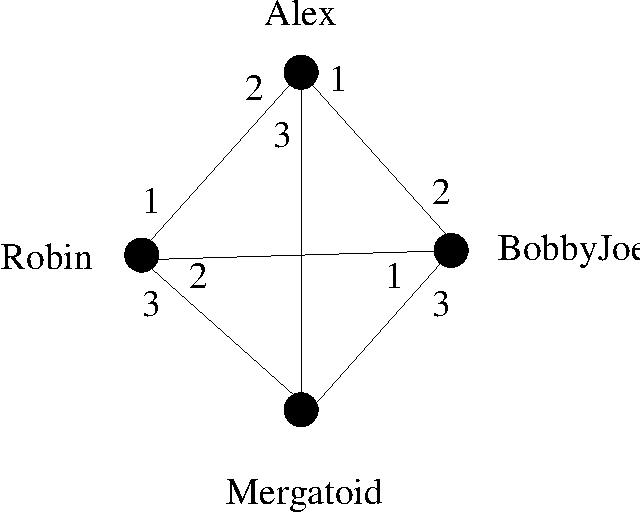
\includegraphics[height=2.3in]{figures/loveTriangle.pdf}
%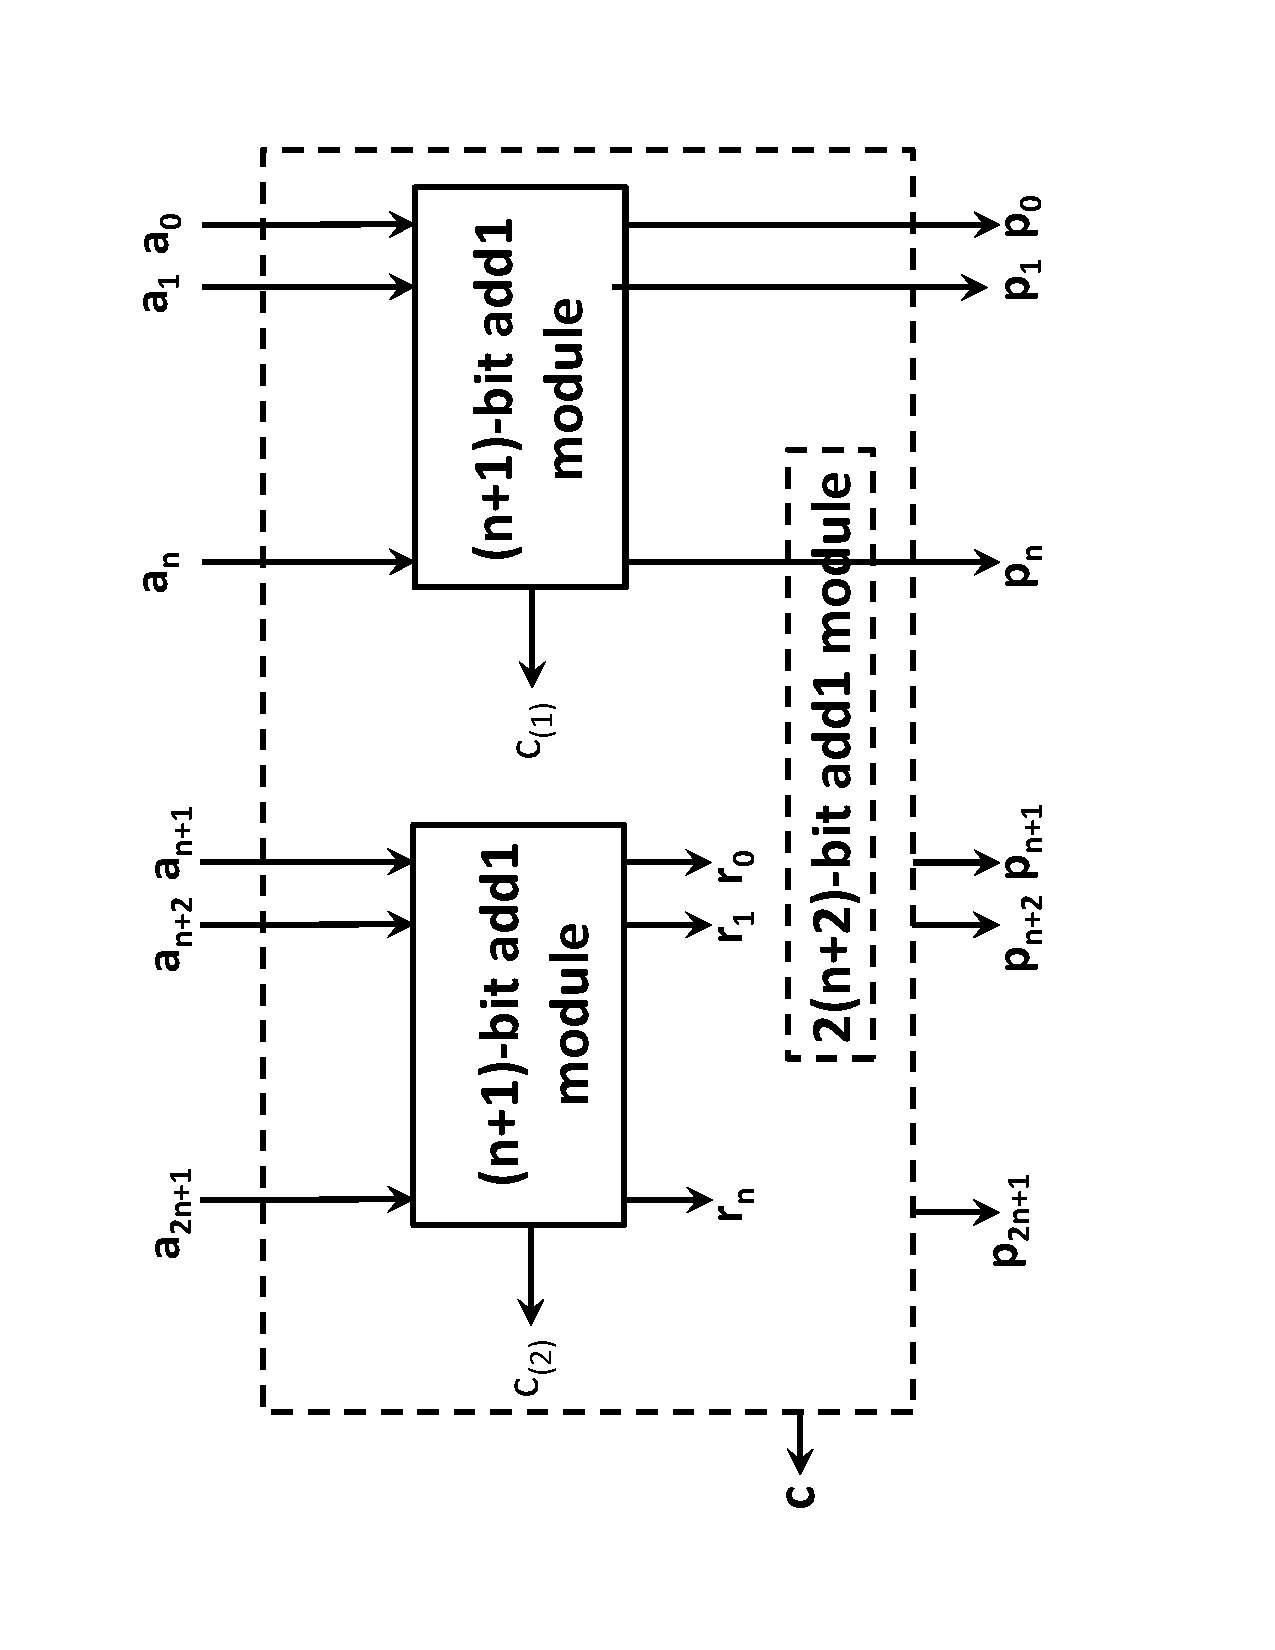
\includegraphics{latex-macros/figures/add1-circuit-diagram.pdf}
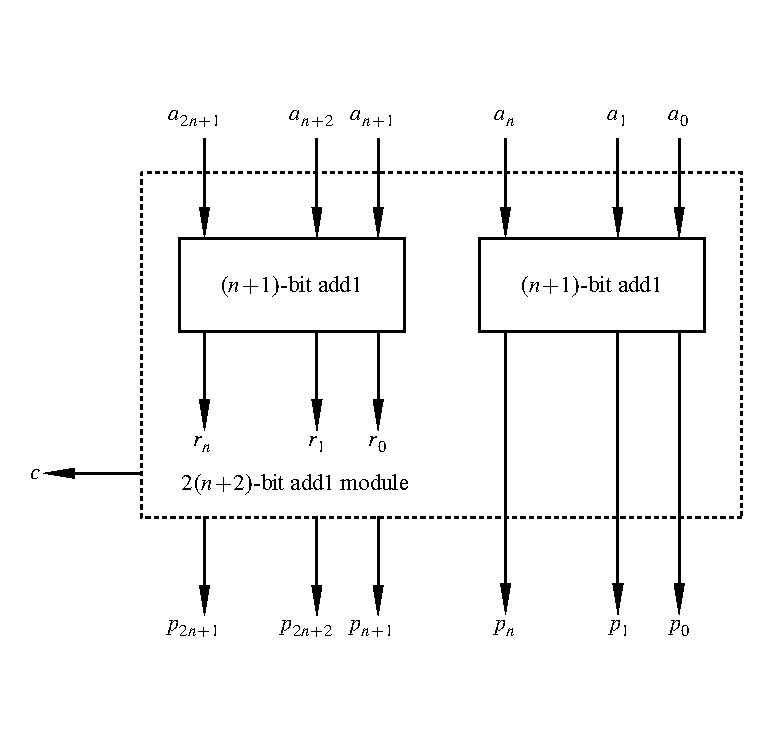
\includegraphics[height=9in]{add1-circuit-diagram.pdf}
\caption{Structure of a Double-size Add1 Module.}
\label{fig:add1}
\end{figure}

%%%%%%%%%%%%%%%%%%%%%%%%%%%%%%%%%%%%%%%%%%%%%%%%%%%%%%%%%%%%%%%%%%%%%
% Problems end here
%%%%%%%%%%%%%%%%%%%%%%%%%%%%%%%%%%%%%%%%%%%%%%%%%%%%%%%%%%%%%%%%%%%%%
\end{document}

